\documentclass[a4paper]{article}

\usepackage[utf8]{inputenc}
\usepackage[T2A]{fontenc}
\usepackage[russian]{babel}

\usepackage{verbatim}
\usepackage{graphicx}
\usepackage{indentfirst}
\usepackage[a4paper,top=2.5cm,bottom=2.5cm,left=2.5cm,right=1cm,head=17pt]{geometry}

\usepackage{tabularx}
\newcolumntype{Y}{>{\centering\arraybackslash}X}

\usepackage{amssymb}
\renewcommand{\le}{\leqslant}
\renewcommand{\ge}{\geqslant}

\usepackage{ifpdf}
\ifpdf
\DeclareGraphicsRule{*}{mps}{*}{}
\fi

\newcounter{algorithm}
\newenvironment{algorithm}[1]{\par\smallskip\noindent\refstepcounter{algorithm}%
  \textbf{Алгоритм \arabic{algorithm}. #1}\begin{enumerate}}{\end{enumerate}}

\newtheorem{define}{Определение}
\renewcommand{\thedefine}{\arabic{define}.}

\newtheorem{theorem}{Теорема}
\renewcommand{\thetheorem}{\arabic{theorem}.}

\renewcommand{\thesection}{\arabic{section}.}

\newcommand{\ticket}[1]{\noindent{\huge{}#1}}

\frenchspacing


\begin{document}
\ticket{2.5. Вычислительная геометрия на плоскости}
\section{Уравнения точек, прямых, окружностей}
\begin{define}
  Евклидово пространство размерности $k$ $E^k$ --- пространство
  кортежей вида $(x_1, \ldots, x_k)$ вещественных чисел $x_i$, $1 \le
  i \le k$.
\end{define}

Расстояние между двумя точками $p_1 = (x_1, \ldots, x_k)$ и $p_2 =
(y_1, \ldots, y_k)$ равно $$d(p_1, p_2) = \left(\sum_{i=1}^k|y_i -
x_i|^2\right)^{1/2}$$

Пусть $p$, $q$ - точки на прямой, $n$ - нормаль к прямой, $d$ -
направляющий вектор прямой.
Рассмотрим основные способы задания прямых на плоскости.
\begin{enumerate}
\item $(1 - \alpha) p + \alpha q, \alpha \in R$, или $p + \alpha d$,
  где $d = q - p$. Этот способ является
  основным средством представления прямых в трехмерном пространстве.
  На плоскости удобен для поиска пересечений прямой с другими
  объектами. В этом случае $n = (d_y, -d_x)$.
\item $y = kx + b$. Здесь $k$ - тангенс угла наклона, $b$ -
  пересечение прямой с осью ординат. Используется в некоторых
  геометрических преобразованиях двойственности. Существенный
  недостаток --- невозможность представить в таком виде вертикальные
  прямые.
\item $n \cdot p = -C$. Если $n=(A, B)$, то уравнение можно записать в
  виде $Ap_x + Bp_y + C=0$. Неравенства $Ap_x + Bp_y + C \le 0$ и
  $Ap_x + Bp_y + C \ge 0$ задают полуплоскости, на которые прямая
  делит плоскость координат. Расстояние от начала координат до прямой
  равно $|C / \|n\||$. Расстояние от точки $q$ до прямой --- $(n \cdot
  q + C) / \|n\|$.
\end{enumerate}

Точки $p$, принадлежащие окружности на плоскости с центром в точке
$c$ и радиусом $r$, удовлетворяют уравнению $d(p, c) \le r$, что можно
записать в форме $(p_x - c_x)^2 + (p_y - c_y)^2 \le r^2$.

\section{Выпуклые оболочки, алгоритмы построения}
\begin{define}
  Многоугольник называется выпуклым, если отрезок, соединяющий любые
  его две точки, принадлежит многоугольнику.
\end{define}
\begin{define}
  Точка принадлежит границе многоугольника, если любая её окрестность
  содержит точки, как принадлежащие, так и не принадлежащие
  многоугольнику.
\end{define}
\begin{define}
  Пусть в n-мерном пространстве задано $k$ различных точек $p_1, \ldots, p_k$.
  Множество точек $p$, таких, что: $p = a_1p_1 + a_2p_2 + \ldots +
  a_kp_k$, где $a_j \in R$,
  $a_j \ge 0$ , $a_1 + a_2 + \ldots a_k = 1$ называется выпуклым множеством,
  порожденным точками $p_1, \ldots, p_k$, а $p$ называется выпуклой комбинацией
  точек $p_1, \ldots, p_k$.
\end{define}
\begin{define}
  Выпуклой оболочкой (convex hull) множества M точек n-мерного
  пространства называется наименьшее выпуклое множество, содержащее M,
  и обозначается conv(M).
\end{define}

Опишем классические алгоритмы построения выпуклой оболочки множества
точек.

\begin{algorithm}{Метод обхода Джарвиса (``заворачивание подарка'').}
\item Выбираем самую левую точку множества $p_0$. Эта точка заведомо
  является вершиной выпуклой оболочки.
\item Находим точку множества $p_1$, имеющую наименьший положительный
  полярный угол относительно точки $p_0$ как начала координат.
\item Находим точку множества $p_2$, имеющую наименьший положительный
  полярный угол относительно точки $p_1$ как начала координат.
\item И т. д., пока не достигнем точки $p_0$.
\end{algorithm}

Корректность алгоритма очевидна. Каждая новая вершина определяется за
$O(n)$. В худшем случае, когда все $n$ точек лежат на выпуклой оболочке,
сложность алгоритма $O(n^2$). Если $h$ --- число вершин выпуклой оболочки, то
сложность алгоритма --— $O(hn)$.

\begin{algorithm}{Алгоритм обхода Грэхема.}
\item Найти самую левую нижнюю точку $q$ множества исходных точек.
\item Используя $q$ как начало координат, упорядочить точки множества
  ``лексикографически'': в соответствии с полярным углом и расстоянием
  от $q$.
\item Обход точек. Хранится стек точек $\{p_{i_1}, \ldots,p_{i_k}\}$,
  просмотренных к настоящему времении. Все тройки соседних вершин в
  стеке образуют левый поворот. При рассмотрении очередной точки $p_i$
  возможна одна из следующих ситуаций. Если $p_{i_{k-1}},p_{i_k},p_i$
  образуют левый поворот, то точка $p_i$ просто добавляется на вершину
  стека и индекс $i$ увеличивается на $1$.
  Если $p_{i_{k-1}},p_{i_k},p_i$ образуют правый поворот, $p_{i_k}$ не
  может быть крайней точкой, так как она является внутренней точкой
  $\triangle qp_{i_{k-1}}p_i$. В этом случае нужно удалить вершину
  $p_{i_k}$ из стека и перейти к началу шага.
\item После окончания обхода в стеке будут храниться вершины выпуклой
  оболочки в порядке обхода против часовой стрелки.
\end{algorithm}

В процессе обхода после каждой проверки угла происходит либо удаление
точки и возврат на одну точку, либо продвижение вперед на одну точку.
Так как множество содержит лишь $n$ точек, то продвижение вперед не
может происходить более $n$ раз, как не может быть удалено и более $n$
точек. Таким образом, обход точек выполняется за линейное время.
Сортировка требует времени $O(n\log n)$, поэтому общая сложность
алгоритма --- $O(n\log n)$.

\begin{theorem}
  Задача сортировки сводима за линейное время к задаче построения
  выпуклой оболочки, и, следовательно, для нахождения упорядоченной
  выпуклой оболочки n точек на плоскости требуется время $O(n \log n)$.
\end{theorem}

Чтобы доказать теорему, сопоставим каждому из заданных $n$
положительных чисел $x_1, \ldots, x_n$ точку $(x_i, x_i^2)$. Все эти
точки лежат на параболе $y=x^2$. Выпуклая оболочка полученного
множества будет состоять из списка всех точек этого множества,
упорядоченных по значению абсциссы. Поэтому если бы выпуклую оболочку
можно было найти быстрее чем за $\Omega(n\log n)$, то и задача
сортировки решалась бы быстрее, что неверно.

Можно показать, что точная нижняя оценка времени построения выпуклой
оболочки множества точек --- $O(n\log h)$. Известны алгоритмы,
работающие за это время --- это алгоритмы Kirkpatrick-Seidel'я и Chan'а.

\section{Алгоритмы триангуляции}
\begin{define}
  Триангуляцией называется планарный граф, все внутренние области
  которого являются треугольниками.
\end{define}
\begin{define}
  Задачей построения триангуляции по заданному набору двумерных точек
  называется задача соединения заданных точек непересекающимися
  отрезками так, чтобы образовалась триангуляция.
\end{define}

Задача построения триангуляции по исходному набору точек является
неоднозначной, поэтому возникает вопрос, какая из двух различных
триангуляций лучше.

\begin{define}
  Триангуляция называется оптимальной, если сумма длин всех рёбер
  минимальна среди всех возможных триангуляций, построенных на тех
  же исходных точках.
\end{define}

Задача построения оптимальной триангуляции является NP-полной.
Поэтому для большинства реальных задач
существующие алгоритмы построения оптимальной триангуляции
неприемлемы ввиду слишком высокой трудоёмкости.

При  необходимости  на практике применяют приближенные алгоритмы.
Одним  из  первых был  предложен  следующий  алгоритм  построения
триангуляции.
\begin{algorithm}{Жадный алгоритм построения триангуляции.}
\item Генерируется список всех возможных отрезков, соединяющих пары
  исходных точек, и он сортируется по длинам отрезков.
\item Начиная с самого короткого, последовательно выполняется вставка
  отрезков в триангуляцию. Если отрезок не пересекается с другими
  ранее вставленными отрезками, то он вставляется, иначе он
  отбрасывается.
\end{algorithm}

Заметим, что если все возможные отрезки имеют разную длину, то
результат работы этого алгоритма однозначен, иначе он зависит от
порядка вставки отрезков одинаковой длины.
\begin{define}
  Триангуляция называется жадной, если она построена жадным
  алгоритмом.
\end{define}

Трудоемкость работы жадного алгоритма при некоторых его улуч- шениях
составляет $O(n^2 \log n)$. В связи со столь большой трудоемкостью
на практике он почти не применяется. Кроме оптимальной и жадной
триангуляции, также широко известна триангуляция Делоне, обладающая
рядом практически важных свойств.

\begin{define}
  Говорят, что триангуляция удовлетворяет условию Делоне, если внутрь
  окружности, описанной вокруг любого построенног треугольника, не
  попадает ни одна из заданных точек триангуляции.
\end{define}

\begin{define}
  Триангуляция называется триангуляцией Делоне, ес ли она является
  выпуклой и удовлетворяет условию Делоне.
\end{define}

Многие  алгоритмы  построения  триангуляции  Делоне  используют
следующую теорему.

\begin{figure}
  \begin{tabularx}{\textwidth}{YY}
    \includegraphics{figures-1.ps} & \includegraphics{figures-2.ps} \\
    (а) & (б) \\
  \end{tabularx}
  \caption{Флип при построении триангуляции Делоне. $D$ принадлежит
    описанной окружности $\triangle ABC$, поэтому замена ребра $AC$
    на $BD$ позволяет улучшить триангуляцию.}
  \label{fig:flip}
\end{figure}

\begin{theorem}
  Триангуляцию Делоне можно получить из любой другой триангуляции по
  той же системе точек, последовательно перестраивая пары соседних
  треугольников $\triangle ABC$ и $\triangle BCD$, не удовлетворяющих
  условию Делоне, в пары треугольников $\triangle ABD$ и $\triangle
  ACD$. Такая операция перестроения также часто называется флипом
  (см.~ рис.~\ref{fig:flip}).
\end{theorem}

Данная теорема позволяет строить триангуляцию Делоне последовательно,
построив вначале некоторую триангуляцию, а потом последовательно
улучшая её до выполнения условия Делоне.

\begin{theorem}
Триангуляция  Делоне  обладает  максимальной  суммой
минимальных углов всех своих треугольников среди всех возможных три-
ангуляций.
\end{theorem}

\begin{theorem}
  Триангуляция Делоне обладает минимальной суммой радиусов
  окружностей, описанных около треугольников, среди всех возможных
  триангуляций.
\end{theorem}

Наиболее распространенный алгоритм триангуляции Делоне ---
инкрементальный, т.~е. точки добавляются в триангуляцию
последовательно, модифицируя текущую триангуляцию.
\begin{algorithm}{Алгоритм вставки новой точки в триангуляцию Делоне}
\item Локализация точки, то есть определение существующего
  треугольника в триангуляции, которому принадлежит новая точка. При
  использовании иерархии триангуляций может быть осуществлен за время
  $O(\log n)$.
\item Флип ребер. Каждое новое ребро будет иметь новую точку в
  качестве одного из своих концов, поэтому, требуемое для перестроения
  треугольников, равно $O(d)$, где $d$ --- степень новой вершины
  триангуляции. Так как триангуляция --- планарный граф, то $E(d)=O(1)$.
\end{algorithm}
Таким образом, время работы инкрементального алгоритма построения
триангуляции Делоне --- $O(n\log n)$.

\begin{figure}
  \centering
  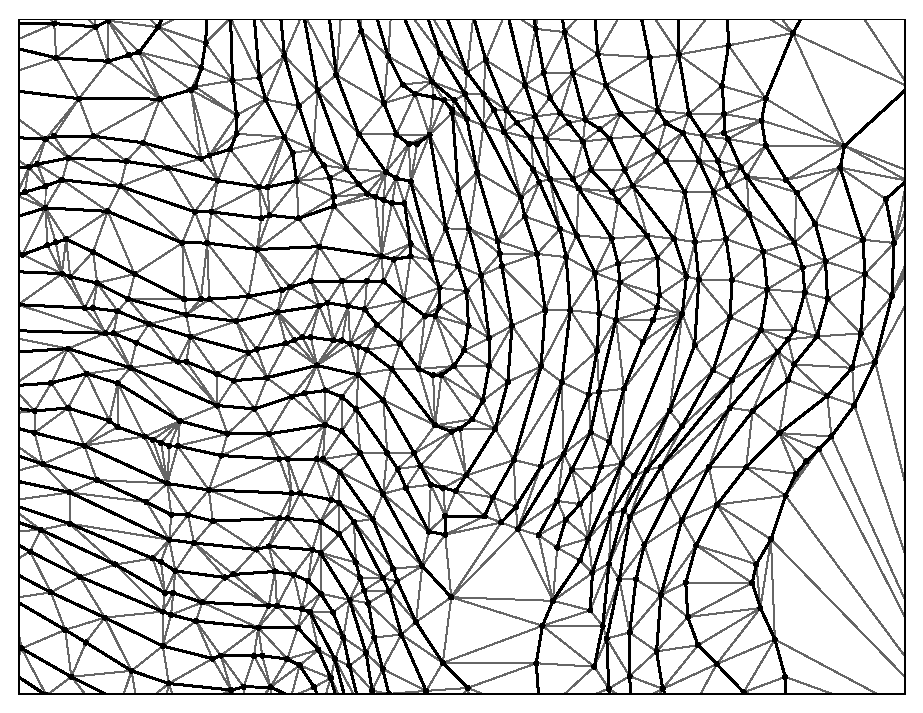
\includegraphics{cdt.ps}
  \caption{Триангуляция Делоне с ограничениями.}
  \label{fig:cdt}
\end{figure}

Возможно задание набора ребер, которые должны входить в триангуляцию
множества точек. В таком случае говорят о задаче триангуляции с
ограничениями. Пример триангуляции Делоне с ограничениями приведен на рис.~\ref{fig:cdt}.

\begin{define}
  Простым многоугольником называется самонепересекающаяся замкнутая
  ломанная.
\end{define}

Триангуляция простого треугольника может быть построена алгоритмом
триангуляции Делоне с ограничениями, однако существуют более простые
алгоритмы триангуляции, не гарантирующие выполнения условия Делоне.

\begin{algorithm}{Триангуляция простого многоугольника за $O(n^2)$}
\item Найти диагональ многоугольника. Это может быть сделано за
 линейное время следующим способом. Рассмотрим многоугольник $\{p_1,
 \ldots, p_n\}$. Пусть $p_k$ --- его выпуклая вершина. Тогда если
 отрезок $p_{k-1}, p_{k+1}$ не пересекает ни одной из сторон
 многоугольника, то он --- искомая диагональ. Иначе диагональю
 является отрезок $p_k,q$, где $q$ --- одна из вершин исходного
 многоугольника, принадлежащая $\triangle p_{k-1}p_kp_{k+1}$.
\item Разбить многоугольник найденной диагональю на два новых
  многоугольника и рекурсивно триангулировать каждый из них.
\end{algorithm}

Триангуляцию простого многоугольника за $On \log n)$ можно
осуществить, разбив его на монотонные многоугольники, а затем
триангулировав за линейное время каждый из них.
Для задачи триангуляции простого многоугольника известен алгоритм,
работающий за время $O(n)$, однако он имеет большую константу и не
применяется на практике.

\section{Задачи регионального поиска}
Задачами регионального поиска называют задачи извлечения или подсчета
геометрических объектов (например, точек, отрезков, прямоугольников),
которые попадают внутрь региона-запроса, представляющего собой стандартную
геометрическую фигуру, произвольно перемещаемую в пространстве.
Как правило, для заданных геометрических объектов на этапе
предобработки строится какая-либо структура данных, позволяющая быстро
отвечать на запросы.

\begin{figure}[t]
  \centering
  \includegraphics{figures-3.ps}
  \caption{$2d$-дерево}
  \label{fig:2d-tree}
\end{figure}


Рассмотрим некоторые примеры задач регионального поиска. Структура
данных $kd$-дерево служит для поиска точек в $k$-мерном пространстве,
попадающих в заданный прямоугольник. Опишем построение и использование
$2d$-дерева.

\begin{algorithm}{Построение $2d$-дерева для множества точек $P$.}
\item Если $P = \{p\}$, то вернуть новый лист дерева с точкой $p$.
\item Разбить множество $P$ на два подмножества $P_1$ и $P_2$.
  Если глубина текущего узла дерева нечетна, то разбиение производится
  вертикальной прямой с абсциссой, равной медиане абсцисс точек из $P$.
  В противном случае разбиение проивзодится горизонтальной прямой с
  ординатой, равной медиане ординат точек $P$.
\item Рекурсивно построить дерево для $P_1$ и $P_2$.
\item Вернуть узел, содержащий прямую разделения, сыновьями которого
  являются деревья для $P_1$ и $P_2$.
\end{algorithm}
Пример $2d$-дерева можно посмотреть на рис.~\ref{fig:2d-tree}.

\begin{theorem}
  $2d$-дерево для множества из $n$ точек может быть построено за время
  $O(n \log n)$, используя $O(n)$ памяти.
\end{theorem}

Запрос точек по прямоугольнику $Q$ осуществляется спуском по дереву.
Каждому узлу дерева соответствует область $R$, которую он покрывает вместе
со своими детьми. Если $Q$ пересекается с $R$, то необходимо сделать
запрос для обоих сыновей этого узла и объединить результаты.

\begin{theorem}
  Поиск точек, попадающих в изоориентированный прямоугольник $Q$,
  выполняется для $2d$-дерева множества $P$, содержащего $n$ точек, за время
  $O(\sqrt n + k$), где $k$ --- количество точек из множества $P$,
  принадлежащих $Q$.
\end{theorem}

Более лучший результат по времени запроса, но худший по памяти, дают
так называемые деревья регионов. Они представляют собой
сбалансированные деревья поиску по абсциссам заданного набора точек, в
каждом узле $Q$ которого содержится сбалансированное дерево поиска по
ординатам точек, принадлежащих поддереву $Q$.

\begin{theorem}
  Дерево регионов для множества из $n$ точек может быть построено за
  время $O(n log n)$, используя $O(n log n)$ памяти. Время запроса по
  прямоугольнику при этом составляет $O(\log n + k)$.
\end{theorem}

\end{document}
